\documentclass[12pt]{amsart}
\usepackage[T1]{fontenc}
\usepackage[utf8]{inputenc}

\usepackage[top=1.95cm, bottom=1.95cm, left=2.35cm, right=2.35cm]{geometry}

\usepackage{hyperref}
\usepackage{enumitem}
\usepackage{tcolorbox}
\usepackage{multicol}
\usepackage{fancyvrb}
\usepackage{amsmath}
\usepackage[french]{babel}

\usepackage{lymath}


\newtheorem{fact}{Fait}
\newtheorem{example}{Exemple}
\newtheorem*{proof*}{Preuve}

\setlength\parindent{0pt}


\DeclareMathOperator{\taille}{\text{\normalfont\texttt{taille}}}

\newcommand\sqseq[2]{\fbox{$#1$}_{\,\,#2}}


\DefineVerbatimEnvironment{rawcode}%
	{Verbatim}%
	{tabsize=4,%
	 frame=lines, framerule=0.3mm, framesep=2.5mm}
	 
	 
	 
\begin{document}

\title{BROUILLON - Sommer les carrés des chiffres d'un naturel}
\author{Christophe BAL}
\date{6 Juin 2018 -- 9 Déc. 2018}

\maketitle

\begin{center}
	\itshape
	Document, avec son source \LaTeX, disponible sur la page
	
	\url{https://github.com/bc-writing/drafts}.
\end{center}



\setcounter{tocdepth}{1}
\tableofcontents



\section{Faire une tête au carré à tous les entiers naturels}

Voici un procédé facile à faire à l'aide d'une calculatrice.


\medskip

\begin{tcolorbox}
	Considérons un entier naturel $n$.
	
	\begin{itemize}[label = \small\textbullet]
		\item Élevons chacun des chiffres de $n$ au carré.
		
		\item Additionnons tous ces carrés. Notons $n$ cette somme.
		
		\item Retournons au premier point.
	\end{itemize}

	On peut alors étudier ce processus qui peut être infini a priori.
\end{tcolorbox}

Voici deux exemples instructifs pour la suite.


\begin{example}
	Pour $n = 19$, nous obtenons :
	\begin{itemize}[label=\textbullet]
		\item $1^2 + 9^2 = 82$
		\item $8^2 + 2^2 = 68$
		\item $6^2 + 8^2 = 100$
		\item $1^2 + 0^2 + 0^2 = 1$ $\rightarrow$ Rien de nouveau à attendre.
	\end{itemize}
\end{example}


\begin{example}
	Pour $n = 1\,234\,567\,890$, après $1^2 + 2^2 + 3^2 + 4^2 + 5^2 + 6^2 + 7^2 + 8^2 + 9^2 + 0^2 = 285$ nous obtenons :
	\vspace{-.7em}
	\begin{multicols}{2}
		\begin{itemize}[label=\textbullet]
			\item $2^2 + 8^2 + 5^2 = 93$
			\item $9^2 + 3^2 = 90$
			\item $9^2 + 0^2 = 81$
			\item $8^2 + 1^2 = 65$
			\item $6^2 + 5^2 = 61$
			\item $6^2 + 1^2 = 37$
			\item $3^2 + 7^2 = 58$
		\end{itemize}
		\columnbreak
		\begin{itemize}[label=\textbullet]
			\item $5^2 + 8^2 = 89$
			\item $8^2 + 9^2 = 145$
			\item $1^2 + 4^2 + 5^2 = 42$
			\item $4^2 + 2^2 = 20$
			\item $2^2 + 0^2 = 4$
			\item $4^2 = 16$ 
			\item $1^2 + 6^2 = 37$ $\rightarrow$ Dèjà rencontré.
		\end{itemize}
	\end{multicols}
\end{example}

Dans le 1\ier{} cas, au bout d'un moment le procédé ne produit que des $1$. Ce sera par exemple le cas dès que l'on commence avec une puissance de $10$.
Quant au 2\ieme{} exemple, il montre que le mieux que l'on puisse espérer c'est que le procédé devienne périodique à partir d'un moment \emph{(on parle de phénomène ultimement périodique)}.


\medskip

On peut explorer le comportement de ce procédé sur plusieurs valeurs grâce à un programme. Voici un code possible non optimisé écrit en Python 3.7 qui prend un peu de temps pour vérifier que pour tous les naturels $n \in \ZintervalC{1}{10^6}$, le procédé devient ultimement périodique.

\begin{rawcode}
NMAX    = 10**6
MAXLOOP = 10**20

for n in range(1, NMAX + 1):
    nbloops = 0
    results = []

    while nbloops < MAXLOOP and n not in results:
        nbloops += 1
        results.append(n)
        n = sum(int(d)**2 for d in str(n))

    if n not in results:
        print(f"Test raté pour n = {n}.")

print("Tests finis.")
\end{rawcode}

\medskip

Une fois lancé, le code précédent affiche juste \verb+Tests finis+.
Il reste à voir ce qu'il se passe dans le cas général. La section qui suit démontre que pour tout naturel $n$, le procédé sera toujours ultimement périodique.




\section{Une preuve}\label{proof}

On introduit les notations suivantes.
\begin{itemize}[label = \textbullet]
	\item Pour un naturel $n$,
	$\displaystyle      n =  \left[ \, c_{d-1} c_{d-2} \cdots c_1 c_0 \, \right]_{10} 
	\stackrel{\text{def}}{=} \sum_{k=0}^{d-1} c_k 10^k$,
	avec $c_{d-1} \neq 0$, désigne l'écriture décimale propre de $n$.
	
	\item On pose enuite
	$\displaystyle sq(n) = \sum_{k=0}^{d-1} (c_k)^2$
	et
	$\taille(n) = d$ sera appelé \emph{\og taille de $n$ \fg}.


	\item Pour $(n \,; k) \in \NN^2$, on définit 
	$  \sqseq{n}{0} = n$
	et
	$  \sqseq{n}{k} = sq^k(n)
	\stackrel{\text{def}}{=} sq \,\circ sq \,\circ \cdots \,\circ sq(n)$ avec $(k-1)$ compositions si $k > 0$.
	
	
	\smallskip\noindent
	Autrement dit, nous avons
	$\sqseq{n}{0} = n$
	et
	$\sqseq{n}{k+1} = sq \left( \, \sqseq{n}{k} \right)$.


	\item Enfin on note
	$V_n = \geneset{ \, \sqseq{n}{k} \, | \, k \in \NN }$
	l'ensemble des valeurs prises par la suite $\left( \, \sqseq{n}{k} \right)_k$.
\end{itemize}



\bigskip

\begin{fact}
	$\forall n \in \NN$, $sq(n) \leqslant 81 d$ où $d = \taille(n)$.
\end{fact}

\begin{proof*}
	Si $n = \left[ \, c_{d-1} c_{d-2} \cdots c_1 c_0 \, \right]_{10}$
	alors 
	$\displaystyle sq(n) = \sum_{k=0}^{d-1} (c_k)^2 \leqslant \sum_{k=0}^{d-1} 9^2 = 81 d $.
\end{proof*}




\medskip

\begin{fact}\label{magicmajo}
	$\forall n \in \NN$, notant $d = \taille(n)$, nous avons les résultats suivants :
	
	\begin{enumerate}
		\item Si $d \geqslant 4$ alors $sq(n) < n$.
		
		\item Si $d \leqslant 3$ alors $sq(n) < 10^3$.
	\end{enumerate}
\end{fact}

\begin{proof*}
	Comme $n \geqslant 10^{d-1}$ et compte tenu du fait précédent, nous cherchons à comparer $10^{d-1}$ et $81d$.
	Pour cela, regardons ce qu'il se passe pour les premières valeurs de $d$.

	\smallskip
	\begin{center}
		\begin{tabular}{|r|c|c|c|c|c|}
			\hline
				$d$        & $1$  & $2$   & $3$   & $4$    & $5$        \\
			\hline
				$10^{d-1}$ & $1$  & $10$  & $100$ & $1000$ & $10\,000$  \\
			\hline
				$81d$      & $81$ & $162$ & $243$ & $324$  & $405$      \\
			\hline
		\end{tabular}
	\end{center}
	\smallskip
	
	Or lorsque $d \geqslant 2$ augmente de $1$, alors $81d$ augmente de $81$ tandis que $10^{d-1}$ augmente d'au moins $100$.
	Nous en déduisons que $n \geqslant 10^{d-1} > 81d \geqslant sq(n)$ , d'où $n > sq(n)$ , dès que $d \geqslant 4$.
	Ceci prouve le 1\ier{} point.
	Pour les fans de Nicolas B.
	\footnote{
		Alias Nicolas BOURBAKI.
	}, 
	voir la preuve \cpageref{magicmajo-proof} du fait \ref{magicmajo} qui traite le cas d'une puissance quelconque.


	\bigskip
	
	Le 2nd point pour $d \leqslant 3$ découle directement de $sq(999) = 243$.
\end{proof*}




\medskip

\begin{fact}
	$\forall n \in \NN$, l'ensemble $V_n$ est fini et donc la suite $\left( \, \sqseq{n}{k} \right)_{k \in \NN}$ est ultimement périodique, i.e. périodique à partir d'un certain rang.
\end{fact}

\begin{proof*}
	Le 2nd point dépend directement du 1er point via le principe des tiroirs et la définition récursive de la suite $\left( \, \sqseq{n}{k} \right)_k$.
	
	\medskip
	
	Pour le 1er point, pour $n \leqslant 999$, on a directement $V_n \subset \intervalC{0}{999}$,
	sinon il suffit de montrer que $V_n \subset \intervalC{0}{10^{\taille(n)}}$ pour $n \geqslant 10^4$ via une petite récurrence descendante finie.
\end{proof*}


\section{Coder - Étudier la \og période \fg{} d'un naturel}

Quand il ne se fige pas, le code suivant donne la \textit{\og période \fg} d'un naturel auquel on applique le procédé présenté dans la section \ref{conjecture}.

\begin{rawcode}
n     = 20181209
nmemo = n

results = []

while n not in results:
    results.append(n)
    n = sum(int(d)**2 for d in str(n))

print(f"{nmemo} a la période suivante :")
print(results[results.index(n):])

print()

before = results[:results.index(n)]

if before:
    print("Avant la 1ère période nous avons :")
    print(before)
else:
    print("On commence directement par la période.")
\end{rawcode}

\medskip

Le code précédent, où \verb+n = 20181209+, nous affiche :

\begin{rawcode}
20181209 a la période suivante :
[16, 37, 58, 89, 145, 42, 20, 4]

Avant la 1ère période nous avons :
[20181209, 155, 51, 26, 40]
\end{rawcode}


\medskip

\begin{figure}[t]
	\centering
	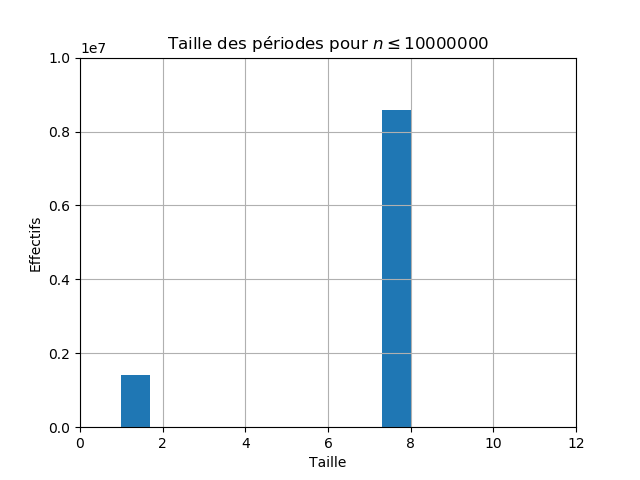
\includegraphics[scale=.9]{squares-int/periods.png}
  	\caption{Histogramme des tailles des périodes}
	\label{histogram}
\end{figure}



\medskip

Amusons-nous maintenant à représenter un histogramme des tailles des \og périodes \fg{}
À l'adresse \url{https://github.com/bc-writing/drafts}, dans le dossier \texttt{squares-int}, vous trouverez le fichier \texttt{squareint-sizeplots.py} qui été utilisé pour obtenir le graphique
\footnote{
	À la même adresse dans le dossier \texttt{squares-int} se trouve l'image \texttt{befores.png} qui est un histogramme des nombres de termes calculés avant l'apparition de la 1\iere{} \emph{\og période \fg{}}.
}.
Le traitement des données a été amélioré pour éviter de refaire des calculs déjà rencontrés \emph{(pour plus de précisions, se reporter aux commentaires du code)}.
Le résultat est donné dans la figure \ref{histogram} \cpageref{histogram}.



\medskip

Le graphique est frappant ! En effet, il semblerait que l'on ait soit des périodes de taille $1$, penser à $0$ et $1$, soit des périodes de taille $8$ comme pour $37 - 58 - 89 - 145 - 42 - 20 - 4 - 16$.
Magie ou coïncidence ? Les résultats de la section \ref{proof}, dont nous allons reprendre les notations, vont nous permettre de le savoir.
Tout d'abord,  d'après le fait \ref{magicmajo}, nous avons $\taille(sq(n)) < \taille(n)$ dès que $\taille(n) \geqslant 4$, donc la périodicité n'arrivera que lorsque $\taille\left( \, \sqseq{n}{k} \right) \leqslant 3$.
De plus, nous savons aussi que $\taille(sq(n)) \leqslant 3$ dès que $\taille(n) \leqslant 3$.
Tout ceci nous permet d'analyser brutalement via un programme ce qu'il se passe pour les périodes des naturels appartenant à $\ZintervalC{0}{999}$. Nous pouvons pour cela utiliser le code suivant, qui n'est absolument pas optimisé mais fait le travail immédiatement.


\newpage

\begin{rawcode}
nmax = 999

periodsfound = []

for n in range(nmax + 1):
    results = []

    while n not in results:
        results.append(n)
        n = sum(int(d)**2 for d in str(n))

    period = results[results.index(n):]

    if period not in periodsfound:
        periodsfound.append(period)

for oneperiod in periodsfound:
    print(oneperiod)
\end{rawcode}



\medskip

Le code précédent nous fournit toutes les périodes possibles.


\newpage

\begin{rawcode}
[0]
[1]
[4, 16, 37, 58, 89, 145, 42, 20]
[37, 58, 89, 145, 42, 20, 4, 16]
[89, 145, 42, 20, 4, 16, 37, 58]
[16, 37, 58, 89, 145, 42, 20, 4]
[20, 4, 16, 37, 58, 89, 145, 42]
[58, 89, 145, 42, 20, 4, 16, 37]
[42, 20, 4, 16, 37, 58, 89, 145]
[145, 42, 20, 4, 16, 37, 58, 89]
\end{rawcode}


\medskip

Et là cela devient joli car nous notons au passage que trois types de périodes : 
\verb+[0]+, \verb+[1]+ et
\verb+[4, 16, 37, 58, 89, 145, 42, 20]+ avec toutes ses \emph{\og permutées circulaires \fg}.

\end{document}
